\documentclass[]{article}
\usepackage{lmodern}
\usepackage{amssymb,amsmath}
\usepackage{ifxetex,ifluatex}
\usepackage{fixltx2e} % provides \textsubscript
\ifnum 0\ifxetex 1\fi\ifluatex 1\fi=0 % if pdftex
  \usepackage[T1]{fontenc}
  \usepackage[utf8]{inputenc}
\else % if luatex or xelatex
  \ifxetex
    \usepackage{mathspec}
  \else
    \usepackage{fontspec}
  \fi
  \defaultfontfeatures{Ligatures=TeX,Scale=MatchLowercase}
\fi
% use upquote if available, for straight quotes in verbatim environments
\IfFileExists{upquote.sty}{\usepackage{upquote}}{}
% use microtype if available
\IfFileExists{microtype.sty}{%
\usepackage{microtype}
\UseMicrotypeSet[protrusion]{basicmath} % disable protrusion for tt fonts
}{}
\usepackage[margin=1in]{geometry}
\usepackage{hyperref}
\hypersetup{unicode=true,
            pdftitle={Lab 8 Regression},
            pdfauthor={Chen Wang, Junke Wang, Zhuozhi Xiong},
            pdfborder={0 0 0},
            breaklinks=true}
\urlstyle{same}  % don't use monospace font for urls
\usepackage{color}
\usepackage{fancyvrb}
\newcommand{\VerbBar}{|}
\newcommand{\VERB}{\Verb[commandchars=\\\{\}]}
\DefineVerbatimEnvironment{Highlighting}{Verbatim}{commandchars=\\\{\}}
% Add ',fontsize=\small' for more characters per line
\usepackage{framed}
\definecolor{shadecolor}{RGB}{248,248,248}
\newenvironment{Shaded}{\begin{snugshade}}{\end{snugshade}}
\newcommand{\AlertTok}[1]{\textcolor[rgb]{0.94,0.16,0.16}{#1}}
\newcommand{\AnnotationTok}[1]{\textcolor[rgb]{0.56,0.35,0.01}{\textbf{\textit{#1}}}}
\newcommand{\AttributeTok}[1]{\textcolor[rgb]{0.77,0.63,0.00}{#1}}
\newcommand{\BaseNTok}[1]{\textcolor[rgb]{0.00,0.00,0.81}{#1}}
\newcommand{\BuiltInTok}[1]{#1}
\newcommand{\CharTok}[1]{\textcolor[rgb]{0.31,0.60,0.02}{#1}}
\newcommand{\CommentTok}[1]{\textcolor[rgb]{0.56,0.35,0.01}{\textit{#1}}}
\newcommand{\CommentVarTok}[1]{\textcolor[rgb]{0.56,0.35,0.01}{\textbf{\textit{#1}}}}
\newcommand{\ConstantTok}[1]{\textcolor[rgb]{0.00,0.00,0.00}{#1}}
\newcommand{\ControlFlowTok}[1]{\textcolor[rgb]{0.13,0.29,0.53}{\textbf{#1}}}
\newcommand{\DataTypeTok}[1]{\textcolor[rgb]{0.13,0.29,0.53}{#1}}
\newcommand{\DecValTok}[1]{\textcolor[rgb]{0.00,0.00,0.81}{#1}}
\newcommand{\DocumentationTok}[1]{\textcolor[rgb]{0.56,0.35,0.01}{\textbf{\textit{#1}}}}
\newcommand{\ErrorTok}[1]{\textcolor[rgb]{0.64,0.00,0.00}{\textbf{#1}}}
\newcommand{\ExtensionTok}[1]{#1}
\newcommand{\FloatTok}[1]{\textcolor[rgb]{0.00,0.00,0.81}{#1}}
\newcommand{\FunctionTok}[1]{\textcolor[rgb]{0.00,0.00,0.00}{#1}}
\newcommand{\ImportTok}[1]{#1}
\newcommand{\InformationTok}[1]{\textcolor[rgb]{0.56,0.35,0.01}{\textbf{\textit{#1}}}}
\newcommand{\KeywordTok}[1]{\textcolor[rgb]{0.13,0.29,0.53}{\textbf{#1}}}
\newcommand{\NormalTok}[1]{#1}
\newcommand{\OperatorTok}[1]{\textcolor[rgb]{0.81,0.36,0.00}{\textbf{#1}}}
\newcommand{\OtherTok}[1]{\textcolor[rgb]{0.56,0.35,0.01}{#1}}
\newcommand{\PreprocessorTok}[1]{\textcolor[rgb]{0.56,0.35,0.01}{\textit{#1}}}
\newcommand{\RegionMarkerTok}[1]{#1}
\newcommand{\SpecialCharTok}[1]{\textcolor[rgb]{0.00,0.00,0.00}{#1}}
\newcommand{\SpecialStringTok}[1]{\textcolor[rgb]{0.31,0.60,0.02}{#1}}
\newcommand{\StringTok}[1]{\textcolor[rgb]{0.31,0.60,0.02}{#1}}
\newcommand{\VariableTok}[1]{\textcolor[rgb]{0.00,0.00,0.00}{#1}}
\newcommand{\VerbatimStringTok}[1]{\textcolor[rgb]{0.31,0.60,0.02}{#1}}
\newcommand{\WarningTok}[1]{\textcolor[rgb]{0.56,0.35,0.01}{\textbf{\textit{#1}}}}
\usepackage{graphicx}
% grffile has become a legacy package: https://ctan.org/pkg/grffile
\IfFileExists{grffile.sty}{%
\usepackage{grffile}
}{}
\makeatletter
\def\maxwidth{\ifdim\Gin@nat@width>\linewidth\linewidth\else\Gin@nat@width\fi}
\def\maxheight{\ifdim\Gin@nat@height>\textheight\textheight\else\Gin@nat@height\fi}
\makeatother
% Scale images if necessary, so that they will not overflow the page
% margins by default, and it is still possible to overwrite the defaults
% using explicit options in \includegraphics[width, height, ...]{}
\setkeys{Gin}{width=\maxwidth,height=\maxheight,keepaspectratio}
\IfFileExists{parskip.sty}{%
\usepackage{parskip}
}{% else
\setlength{\parindent}{0pt}
\setlength{\parskip}{6pt plus 2pt minus 1pt}
}
\setlength{\emergencystretch}{3em}  % prevent overfull lines
\providecommand{\tightlist}{%
  \setlength{\itemsep}{0pt}\setlength{\parskip}{0pt}}
\setcounter{secnumdepth}{0}
% Redefines (sub)paragraphs to behave more like sections
\ifx\paragraph\undefined\else
\let\oldparagraph\paragraph
\renewcommand{\paragraph}[1]{\oldparagraph{#1}\mbox{}}
\fi
\ifx\subparagraph\undefined\else
\let\oldsubparagraph\subparagraph
\renewcommand{\subparagraph}[1]{\oldsubparagraph{#1}\mbox{}}
\fi

%%% Use protect on footnotes to avoid problems with footnotes in titles
\let\rmarkdownfootnote\footnote%
\def\footnote{\protect\rmarkdownfootnote}

%%% Change title format to be more compact
\usepackage{titling}

% Create subtitle command for use in maketitle
\providecommand{\subtitle}[1]{
  \posttitle{
    \begin{center}\large#1\end{center}
    }
}

\setlength{\droptitle}{-2em}

  \title{Lab 8 Regression}
    \pretitle{\vspace{\droptitle}\centering\huge}
  \posttitle{\par}
    \author{Chen Wang, Junke Wang, Zhuozhi Xiong}
    \preauthor{\centering\large\emph}
  \postauthor{\par}
      \predate{\centering\large\emph}
  \postdate{\par}
    \date{due 11/27/19}


\begin{document}
\maketitle

\hypertarget{together-as-a-class}{%
\section{Together as a class:}\label{together-as-a-class}}

We are first going to install and load packages that we will need.

\begin{enumerate}
\def\labelenumi{\arabic{enumi}.}
\tightlist
\item
  Install and load both the \texttt{modelr} package and the
  \texttt{openintro} package. Load the \texttt{tidyverse} package.
\end{enumerate}

For this problem we will be using the data set called \texttt{gpa} from
the \texttt{openintro} package. We are interest in association between
the number of hours of sleep a student gets and their gpas.

\begin{Shaded}
\begin{Highlighting}[]
\KeywordTok{install.packages}\NormalTok{(}\StringTok{"modelr"}\NormalTok{)}
\end{Highlighting}
\end{Shaded}

\begin{verbatim}
## Installing package into '/home/rstudio-user/R/x86_64-pc-linux-gnu-library/3.6'
## (as 'lib' is unspecified)
\end{verbatim}

\begin{Shaded}
\begin{Highlighting}[]
\KeywordTok{install.packages}\NormalTok{(}\StringTok{"openintro"}\NormalTok{)}
\end{Highlighting}
\end{Shaded}

\begin{verbatim}
## Installing package into '/home/rstudio-user/R/x86_64-pc-linux-gnu-library/3.6'
## (as 'lib' is unspecified)
\end{verbatim}

\begin{Shaded}
\begin{Highlighting}[]
\KeywordTok{library}\NormalTok{(modelr)}
\KeywordTok{library}\NormalTok{(openintro)}
\end{Highlighting}
\end{Shaded}

\begin{verbatim}
## Please visit openintro.org for free statistics materials
\end{verbatim}

\begin{verbatim}
## 
## Attaching package: 'openintro'
\end{verbatim}

\begin{verbatim}
## The following objects are masked from 'package:datasets':
## 
##     cars, trees
\end{verbatim}

\begin{Shaded}
\begin{Highlighting}[]
\KeywordTok{library}\NormalTok{(tidyverse)}
\end{Highlighting}
\end{Shaded}

\begin{verbatim}
## -- Attaching packages ------------------------------------------------------------------------------ tidyverse 1.3.0 --
\end{verbatim}

\begin{verbatim}
## v ggplot2 3.2.1     v purrr   0.3.3
## v tibble  2.1.3     v dplyr   0.8.3
## v tidyr   1.0.0     v stringr 1.4.0
## v readr   1.3.1     v forcats 0.4.0
\end{verbatim}

\begin{verbatim}
## -- Conflicts --------------------------------------------------------------------------------- tidyverse_conflicts() --
## x dplyr::filter() masks stats::filter()
## x dplyr::lag()    masks stats::lag()
\end{verbatim}

\begin{enumerate}
\def\labelenumi{\arabic{enumi}.}
\setcounter{enumi}{1}
\tightlist
\item
  Make a scatter plot and describe the association that you see.
\end{enumerate}

\begin{Shaded}
\begin{Highlighting}[]
\NormalTok{gpa }\OperatorTok\StringTok{ }
\StringTok{  }\KeywordTok{ggplot}\NormalTok{(}\KeywordTok{aes}\NormalTok{(}\DataTypeTok{x=}\NormalTok{sleepnight, }\DataTypeTok{y=}\NormalTok{gpa)) }\OperatorTok{+}
\StringTok{  }\KeywordTok{geom_point}\NormalTok{()}
\end{Highlighting}
\end{Shaded}

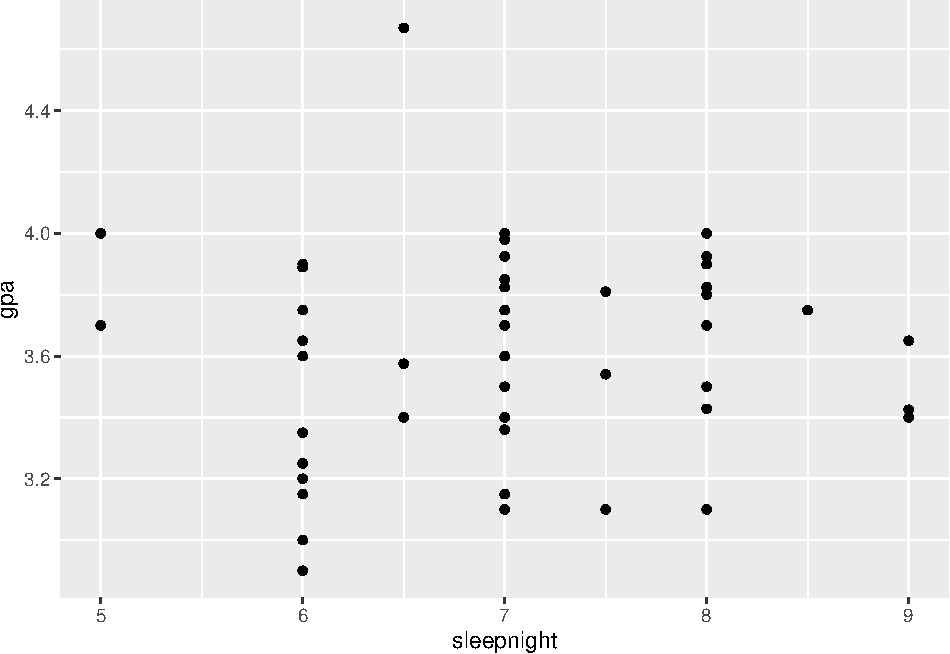
\includegraphics{lab-8-regression_files/figure-latex/unnamed-chunk-3-1.pdf}
It doesn't seem that there is a relationship between hours of sleep and
GPA. We can't tell if there is a positive or a negative trend.

\begin{enumerate}
\def\labelenumi{\arabic{enumi}.}
\setcounter{enumi}{2}
\tightlist
\item
  Create the linear regression model for this relationship between hours
  of sleep and GPA. We are regressing \texttt{gpa} onto
  \texttt{hours\ of\ sleep} Call this model \texttt{gpa\_model}.
\end{enumerate}

\begin{Shaded}
\begin{Highlighting}[]
\NormalTok{gpa_model <-}\StringTok{ }\KeywordTok{lm}\NormalTok{(gpa }\OperatorTok{~}\StringTok{ }\NormalTok{sleepnight, }\DataTypeTok{data=}\NormalTok{gpa)}

\NormalTok{gpa_model }\OperatorTok\StringTok{ }
\StringTok{  }\KeywordTok{summary}\NormalTok{()}
\end{Highlighting}
\end{Shaded}

\begin{verbatim}
## 
## Call:
## lm(formula = gpa ~ sleepnight, data = gpa)
## 
## Residuals:
##      Min       1Q   Median       3Q      Max 
## -0.67898 -0.22123  0.02102  0.21627  1.08110 
## 
## Coefficients:
##             Estimate Std. Error t value Pr(>|t|)    
## (Intercept)  3.46000    0.31819  10.874 4.14e-15 ***
## sleepnight   0.01983    0.04458   0.445    0.658    
## ---
## Signif. codes:  0 '***' 0.001 '**' 0.01 '*' 0.05 '.' 0.1 ' ' 1
## 
## Residual standard error: 0.3381 on 53 degrees of freedom
## Multiple R-squared:  0.003719,   Adjusted R-squared:  -0.01508 
## F-statistic: 0.1978 on 1 and 53 DF,  p-value: 0.6583
\end{verbatim}

\newpage

\begin{enumerate}
\def\labelenumi{\arabic{enumi}.}
\setcounter{enumi}{3}
\tightlist
\item
  Find the correlation of this regression line and give the estimated
  \(\beta\) values.
\end{enumerate}

\begin{Shaded}
\begin{Highlighting}[]
\NormalTok{correlation <-}\StringTok{ }\KeywordTok{sqrt}\NormalTok{(}\FloatTok{0.003719}\NormalTok{)}\CommentTok{#add sign of intercept}
\NormalTok{correlation}
\end{Highlighting}
\end{Shaded}

\begin{verbatim}
## [1] 0.0609836
\end{verbatim}

\begin{Shaded}
\begin{Highlighting}[]
\KeywordTok{cor}\NormalTok{(gpa}\OperatorTok{$}\NormalTok{gpa, gpa}\OperatorTok{$}\NormalTok{sleepnight)}
\end{Highlighting}
\end{Shaded}

\begin{verbatim}
## [1] 0.06098308
\end{verbatim}

the correlation is 0.061. The estimated intercept is 3.46. The estimated
slope is 0.01983.

\begin{enumerate}
\def\labelenumi{\arabic{enumi}.}
\setcounter{enumi}{4}
\tightlist
\item
  Interpret the \(\hat{\beta}\) values. There are 2.
\end{enumerate}

GPA = intercept + slope(hours of sleep)

We can intercept the intercept as us having an estimated GPA of 3.46
when we have 0 hours of sleep.\\
We can interpret the slope as for every 1 extra hour of sleep we get, we
will increase our GPA by 0.01983 points.

\newpage

\begin{enumerate}
\def\labelenumi{\arabic{enumi}.}
\setcounter{enumi}{5}
\tightlist
\item
  Add the predicted values of GPA and the Residuals to the data frame
  \texttt{gpa} using the \texttt{add\_predictions()} and
  \texttt{add\_residuals()} functions from the \texttt{modelr} package.
\end{enumerate}

\begin{Shaded}
\begin{Highlighting}[]
\NormalTok{gpa<-gpa }\OperatorTok\StringTok{ }
\StringTok{  }\KeywordTok{add_predictions}\NormalTok{(gpa_model) }\OperatorTok\StringTok{ }
\StringTok{  }\KeywordTok{add_residuals}\NormalTok{(gpa_model)}
\end{Highlighting}
\end{Shaded}

\begin{enumerate}
\def\labelenumi{\arabic{enumi}.}
\setcounter{enumi}{6}
\tightlist
\item
  Now we want to check the conditions needed to use the least squares
  regression line. Create a qqplot and a residual plots in order to
  check the conditions. Are the conditions meet? Are there any
  outliers?\\
  1 - independence of data\\
  2 - linear relationship of GPA and hours of sleep
\end{enumerate}

4 - constant variability

\begin{Shaded}
\begin{Highlighting}[]
\NormalTok{gpa }\OperatorTok\StringTok{ }
\StringTok{  }\KeywordTok{ggplot}\NormalTok{(}\KeywordTok{aes}\NormalTok{(}\DataTypeTok{sample=}\NormalTok{resid))}\OperatorTok{+}
\StringTok{  }\KeywordTok{geom_qq}\NormalTok{()}
\end{Highlighting}
\end{Shaded}

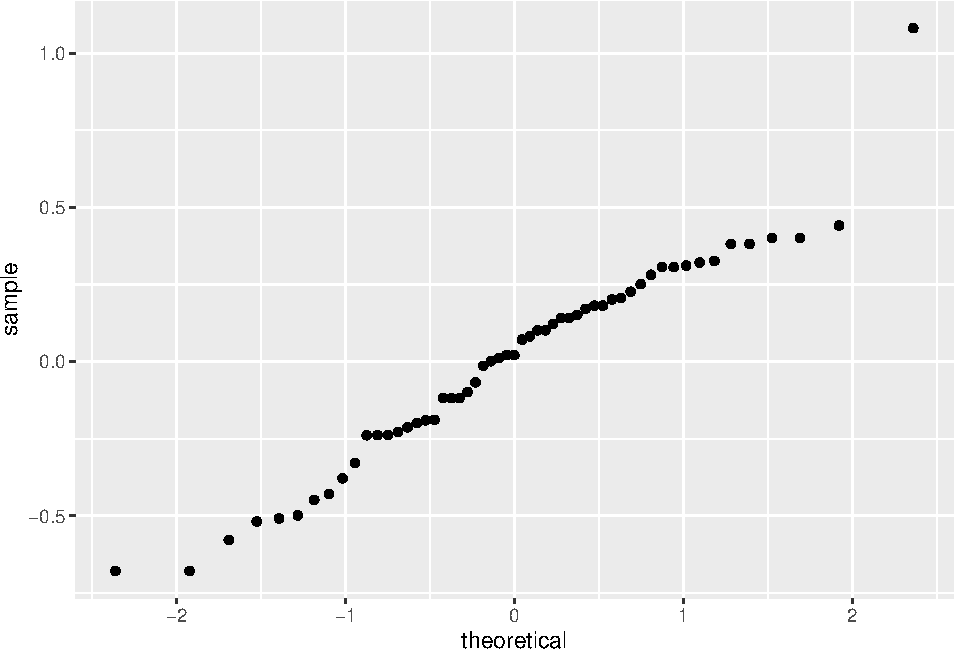
\includegraphics{lab-8-regression_files/figure-latex/unnamed-chunk-7-1.pdf}

\begin{Shaded}
\begin{Highlighting}[]
\NormalTok{gpa }\OperatorTok\StringTok{ }
\StringTok{  }\KeywordTok{ggplot}\NormalTok{(}\KeywordTok{aes}\NormalTok{(}\DataTypeTok{x=}\NormalTok{sleepnight,}\DataTypeTok{y=}\NormalTok{resid))}\OperatorTok{+}
\StringTok{  }\KeywordTok{geom_point}\NormalTok{()}\OperatorTok{+}
\StringTok{  }\KeywordTok{geom_hline}\NormalTok{(}\DataTypeTok{yintercept=}\DecValTok{0}\NormalTok{)}
\end{Highlighting}
\end{Shaded}

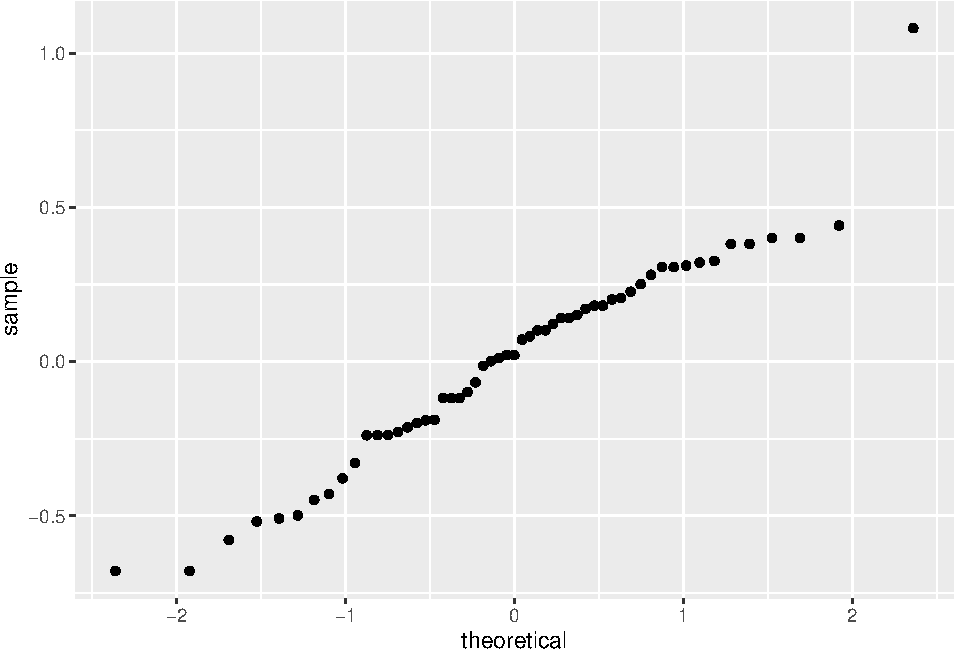
\includegraphics{lab-8-regression_files/figure-latex/unnamed-chunk-8-1.pdf}

All of our assumptions check out. We can use linear regression.

\newpage

\begin{enumerate}
\def\labelenumi{\arabic{enumi}.}
\setcounter{enumi}{7}
\tightlist
\item
  Conduct a hypothesis test to see if there is an association between
  how much sleep a student gets and their GPA. What can we conclude?
\end{enumerate}

\(H_0: \beta_1 = 0\)\\
(We assume the slope is 0. Hours of sleep and GPA have no linear
relationship.)\\
\(H_0: \beta_1\ne0\)\\
(We want to prove that the slope is not 0. That hours of sleep and GPA
have a linear relationship of some kind.)

\begin{Shaded}
\begin{Highlighting}[]
\NormalTok{gpa_model }\OperatorTok\StringTok{ }
\StringTok{  }\KeywordTok{summary}\NormalTok{()}
\end{Highlighting}
\end{Shaded}

\begin{verbatim}
## 
## Call:
## lm(formula = gpa ~ sleepnight, data = gpa)
## 
## Residuals:
##      Min       1Q   Median       3Q      Max 
## -0.67898 -0.22123  0.02102  0.21627  1.08110 
## 
## Coefficients:
##             Estimate Std. Error t value Pr(>|t|)    
## (Intercept)  3.46000    0.31819  10.874 4.14e-15 ***
## sleepnight   0.01983    0.04458   0.445    0.658    
## ---
## Signif. codes:  0 '***' 0.001 '**' 0.01 '*' 0.05 '.' 0.1 ' ' 1
## 
## Residual standard error: 0.3381 on 53 degrees of freedom
## Multiple R-squared:  0.003719,   Adjusted R-squared:  -0.01508 
## F-statistic: 0.1978 on 1 and 53 DF,  p-value: 0.6583
\end{verbatim}

Our t-statistics is 0.445, our p-value is 0.658. Because our p-value is
greater than 0.05, we fail to reject the null hypothesis, we cannot say
there is a linear relationship between hours of sleep and GPA.

\newpage

\hypertarget{on-your-own}{%
\section{On your own:}\label{on-your-own}}

In this problem, we will be using the \texttt{babies} data set from the
\texttt{openintro} package. information about the data set can be found
by running the following code in an \texttt{r} chunk: \texttt{?babies}.
We are interested in finding out how the length of
gestation(\texttt{gestation}), the age of the mother(\texttt{age}), the
height of the mother(\texttt{height}), the mother's
weight(\texttt{weight}), and whether or not this was the mother's first
pregnacy (\texttt{parity}) are related to how much the baby will weight
at birth (\texttt{bwt}).

1.Load the data and save it as \texttt{baby}.

\begin{Shaded}
\begin{Highlighting}[]
\NormalTok{baby <-}\StringTok{ }\NormalTok{babies}
\end{Highlighting}
\end{Shaded}

\begin{enumerate}
\def\labelenumi{\arabic{enumi}.}
\setcounter{enumi}{1}
\tightlist
\item
  Create the linear regression model that regresses \texttt{bwt} the
  variables mentioned above. Print out the summary.
\end{enumerate}

\begin{Shaded}
\begin{Highlighting}[]
\NormalTok{baby_model <-}\StringTok{ }\KeywordTok{lm}\NormalTok{(bwt }\OperatorTok{~}\StringTok{ }\NormalTok{gestation }\OperatorTok{+}\StringTok{ }\NormalTok{age }\OperatorTok{+}\StringTok{ }\NormalTok{height }\OperatorTok{+}\StringTok{ }\NormalTok{weight }\OperatorTok{+}\StringTok{ }\NormalTok{parity, }\DataTypeTok{data=}\NormalTok{ baby)}

\NormalTok{baby_model }\OperatorTok\StringTok{ }
\StringTok{  }\KeywordTok{summary}\NormalTok{()}
\end{Highlighting}
\end{Shaded}

\begin{verbatim}
## 
## Call:
## lm(formula = bwt ~ gestation + age + height + weight + parity, 
##     data = baby)
## 
## Residuals:
##     Min      1Q  Median      3Q     Max 
## -54.569 -10.506   0.453  10.063  54.285 
## 
## Coefficients:
##              Estimate Std. Error t value Pr(>|t|)    
## (Intercept) -86.59435   14.75733  -5.868 5.73e-09 ***
## gestation     0.46579    0.02992  15.568  < 2e-16 ***
## age           0.05233    0.08820   0.593   0.5531    
## height        1.04614    0.21064   4.967 7.82e-07 ***
## weight        0.06564    0.02584   2.540   0.0112 *  
## parity       -2.96394    1.16403  -2.546   0.0110 *  
## ---
## Signif. codes:  0 '***' 0.001 '**' 0.01 '*' 0.05 '.' 0.1 ' ' 1
## 
## Residual standard error: 16.35 on 1178 degrees of freedom
##   (52 observations deleted due to missingness)
## Multiple R-squared:  0.2106, Adjusted R-squared:  0.2072 
## F-statistic: 62.84 on 5 and 1178 DF,  p-value: < 2.2e-16
\end{verbatim}

\begin{enumerate}
\def\labelenumi{\arabic{enumi}.}
\setcounter{enumi}{2}
\item
  Interpret the coefficients for \texttt{gestation} and
  \texttt{parity}.\\
  The coefficient for gestination is 0.46579, which means when other
  explanatory variables don't change, and only gestination increases by
  1 unit, the weight of baby at birth will increase by 0.46579 unit.\\
  The coefficient for parity is -2.96394, which means when other
  explanatory variables don't change, and only parity increases by 1
  unit, the weight of baby at birth will decrease by 2.96394 units.
\item
  Does the intercept value have any meaning in context?\\
  Theoretically, the intercept value means when gestation, age, height,
  weight and parity are all 0, then the weight of the baby will
  -86,59435. But since these factors can not be 0, and baby's weight can
  not be negative, so the intercept value doesn't have meaning in
  context.
\item
  What is the Multiple \(R^2\) value for this model.
\end{enumerate}

\begin{Shaded}
\begin{Highlighting}[]
\NormalTok{baby_model }\OperatorTok\StringTok{ }
\StringTok{  }\KeywordTok{summary}\NormalTok{()}
\end{Highlighting}
\end{Shaded}

\begin{verbatim}
## 
## Call:
## lm(formula = bwt ~ gestation + age + height + weight + parity, 
##     data = baby)
## 
## Residuals:
##     Min      1Q  Median      3Q     Max 
## -54.569 -10.506   0.453  10.063  54.285 
## 
## Coefficients:
##              Estimate Std. Error t value Pr(>|t|)    
## (Intercept) -86.59435   14.75733  -5.868 5.73e-09 ***
## gestation     0.46579    0.02992  15.568  < 2e-16 ***
## age           0.05233    0.08820   0.593   0.5531    
## height        1.04614    0.21064   4.967 7.82e-07 ***
## weight        0.06564    0.02584   2.540   0.0112 *  
## parity       -2.96394    1.16403  -2.546   0.0110 *  
## ---
## Signif. codes:  0 '***' 0.001 '**' 0.01 '*' 0.05 '.' 0.1 ' ' 1
## 
## Residual standard error: 16.35 on 1178 degrees of freedom
##   (52 observations deleted due to missingness)
## Multiple R-squared:  0.2106, Adjusted R-squared:  0.2072 
## F-statistic: 62.84 on 5 and 1178 DF,  p-value: < 2.2e-16
\end{verbatim}

We can see that multiple \(R^2\) for this model is 0.2106.

\newpage

\begin{enumerate}
\def\labelenumi{\arabic{enumi}.}
\setcounter{enumi}{5}
\tightlist
\item
  Add the residuals and predicted values to the data frame.
\end{enumerate}

\begin{Shaded}
\begin{Highlighting}[]
\NormalTok{baby <-}\StringTok{ }\NormalTok{baby }\OperatorTok\StringTok{ }
\StringTok{  }\KeywordTok{add_predictions}\NormalTok{(baby_model) }\OperatorTok\StringTok{ }
\StringTok{  }\KeywordTok{add_residuals}\NormalTok{(baby_model)}
\end{Highlighting}
\end{Shaded}

\begin{enumerate}
\def\labelenumi{\arabic{enumi}.}
\setcounter{enumi}{6}
\tightlist
\item
  Create a residual plot and a qqplot. Comment on whether or not the
  conditions are met to use the model you found in part 2.\\
  The conditions include:\\
  1 - independence of data\\
  2 - linear relationship\\
  3 - normality of residuals\\
  4 - constant variability
\end{enumerate}

\begin{Shaded}
\begin{Highlighting}[]
\NormalTok{baby }\OperatorTok\StringTok{ }
\StringTok{  }\KeywordTok{ggplot}\NormalTok{(}\KeywordTok{aes}\NormalTok{(}\DataTypeTok{sample=}\NormalTok{resid))}\OperatorTok{+}
\StringTok{  }\KeywordTok{geom_qq}\NormalTok{()}
\end{Highlighting}
\end{Shaded}

\begin{verbatim}
## Warning: Removed 52 rows containing non-finite values (stat_qq).
\end{verbatim}

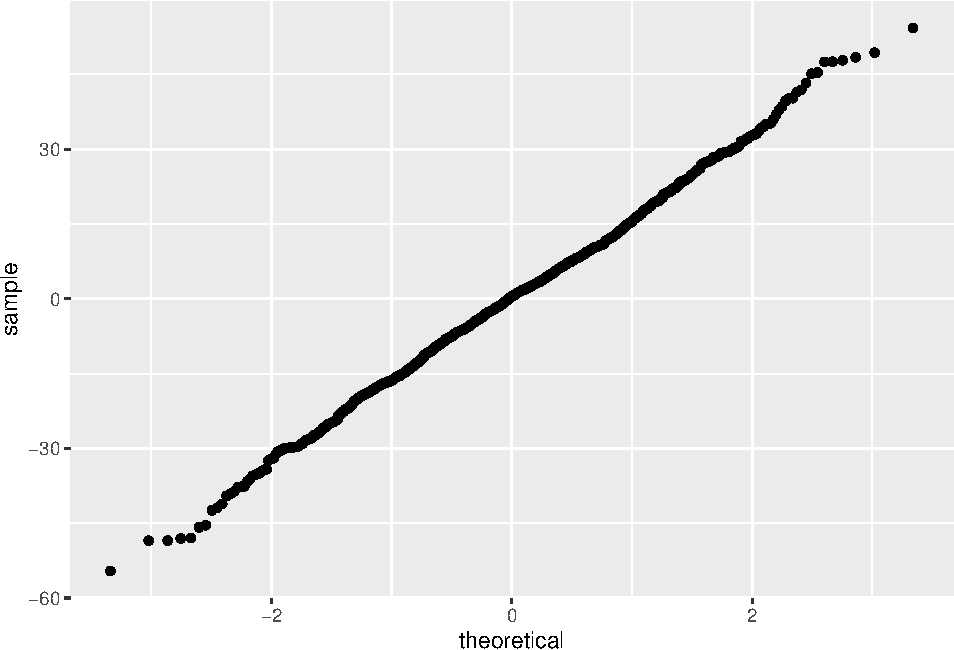
\includegraphics{lab-8-regression_files/figure-latex/unnamed-chunk-14-1.pdf}

\begin{Shaded}
\begin{Highlighting}[]
\NormalTok{baby }\OperatorTok\StringTok{ }
\StringTok{  }\KeywordTok{ggplot}\NormalTok{(}\KeywordTok{aes}\NormalTok{(}\DataTypeTok{x=}\NormalTok{gestation,}\DataTypeTok{y=}\NormalTok{resid))}\OperatorTok{+}
\StringTok{  }\KeywordTok{geom_point}\NormalTok{()}\OperatorTok{+}
\StringTok{  }\KeywordTok{geom_hline}\NormalTok{(}\DataTypeTok{yintercept=}\DecValTok{0}\NormalTok{)}
\end{Highlighting}
\end{Shaded}

\begin{verbatim}
## Warning: Removed 52 rows containing missing values (geom_point).
\end{verbatim}

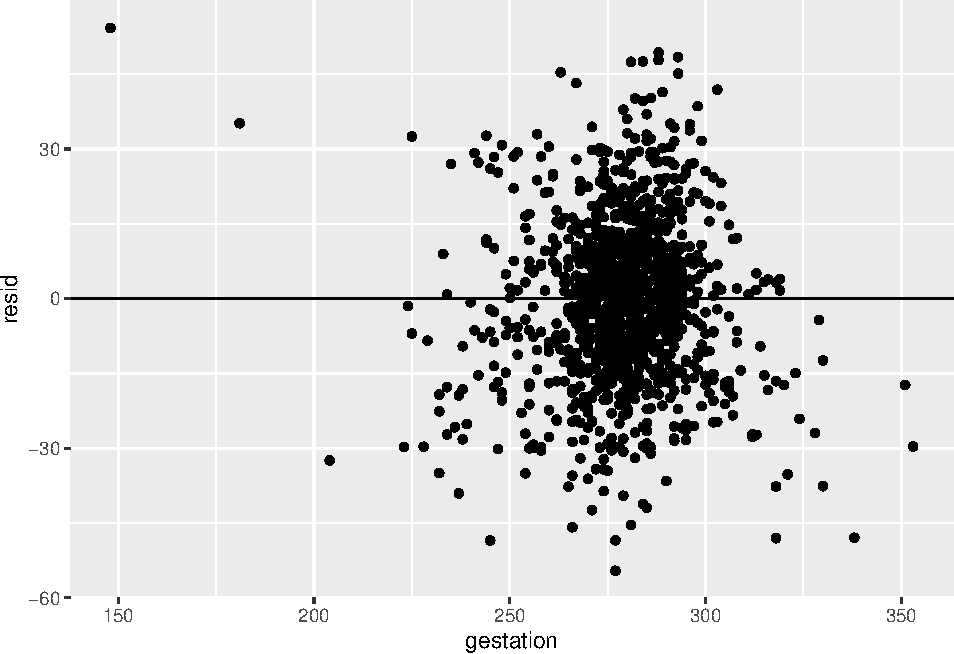
\includegraphics{lab-8-regression_files/figure-latex/unnamed-chunk-15-1.pdf}

\begin{Shaded}
\begin{Highlighting}[]
\NormalTok{baby }\OperatorTok\StringTok{ }
\StringTok{  }\KeywordTok{ggplot}\NormalTok{(}\KeywordTok{aes}\NormalTok{(}\DataTypeTok{x=}\NormalTok{age,}\DataTypeTok{y=}\NormalTok{resid))}\OperatorTok{+}
\StringTok{  }\KeywordTok{geom_point}\NormalTok{()}\OperatorTok{+}
\StringTok{  }\KeywordTok{geom_hline}\NormalTok{(}\DataTypeTok{yintercept=}\DecValTok{0}\NormalTok{)}
\end{Highlighting}
\end{Shaded}

\begin{verbatim}
## Warning: Removed 52 rows containing missing values (geom_point).
\end{verbatim}

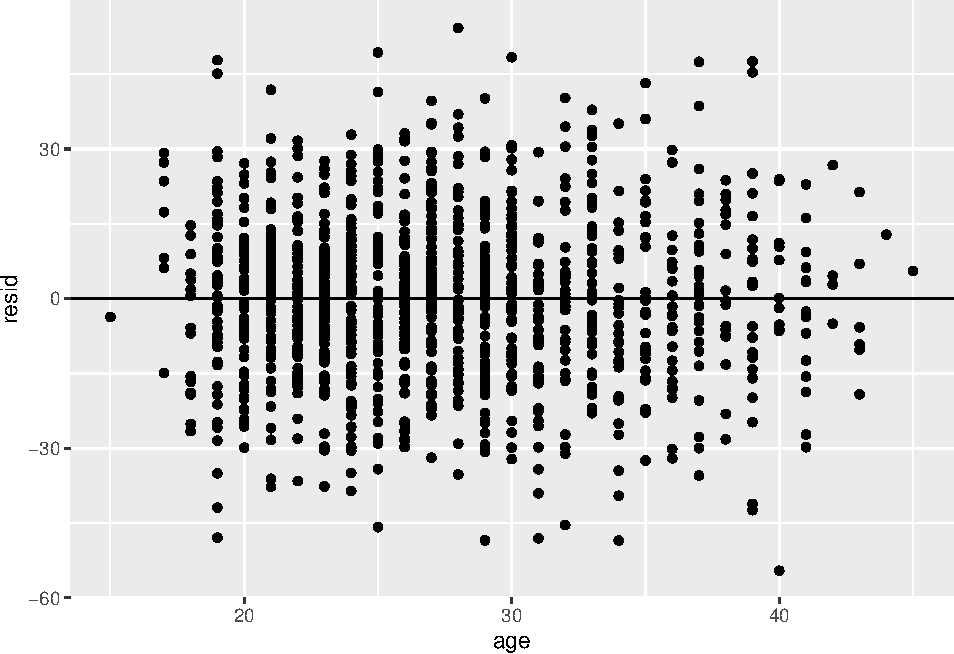
\includegraphics{lab-8-regression_files/figure-latex/unnamed-chunk-16-1.pdf}

\begin{Shaded}
\begin{Highlighting}[]
\NormalTok{baby }\OperatorTok\StringTok{ }
\StringTok{  }\KeywordTok{ggplot}\NormalTok{(}\KeywordTok{aes}\NormalTok{(}\DataTypeTok{x=}\NormalTok{height,}\DataTypeTok{y=}\NormalTok{resid))}\OperatorTok{+}
\StringTok{  }\KeywordTok{geom_point}\NormalTok{()}\OperatorTok{+}
\StringTok{  }\KeywordTok{geom_hline}\NormalTok{(}\DataTypeTok{yintercept=}\DecValTok{0}\NormalTok{)}
\end{Highlighting}
\end{Shaded}

\begin{verbatim}
## Warning: Removed 52 rows containing missing values (geom_point).
\end{verbatim}

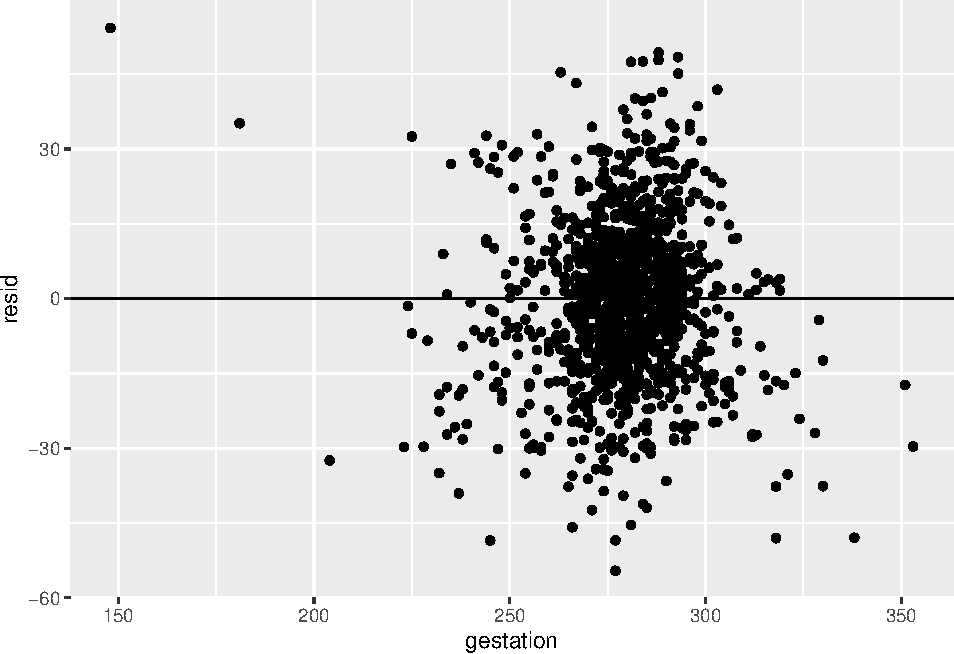
\includegraphics{lab-8-regression_files/figure-latex/unnamed-chunk-17-1.pdf}

\begin{Shaded}
\begin{Highlighting}[]
\NormalTok{baby }\OperatorTok\StringTok{ }
\StringTok{  }\KeywordTok{ggplot}\NormalTok{(}\KeywordTok{aes}\NormalTok{(}\DataTypeTok{x=}\NormalTok{weight,}\DataTypeTok{y=}\NormalTok{resid))}\OperatorTok{+}
\StringTok{  }\KeywordTok{geom_point}\NormalTok{()}\OperatorTok{+}
\StringTok{  }\KeywordTok{geom_hline}\NormalTok{(}\DataTypeTok{yintercept=}\DecValTok{0}\NormalTok{)}
\end{Highlighting}
\end{Shaded}

\begin{verbatim}
## Warning: Removed 52 rows containing missing values (geom_point).
\end{verbatim}

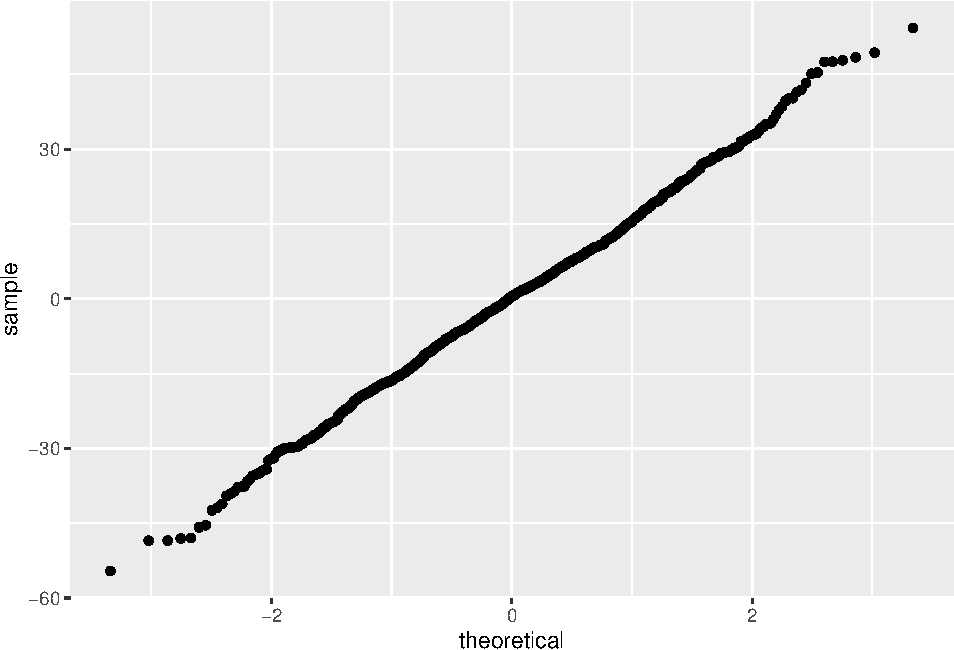
\includegraphics{lab-8-regression_files/figure-latex/unnamed-chunk-18-1.pdf}

\begin{Shaded}
\begin{Highlighting}[]
\NormalTok{baby }\OperatorTok\StringTok{ }
\StringTok{  }\KeywordTok{ggplot}\NormalTok{(}\KeywordTok{aes}\NormalTok{(}\DataTypeTok{x=}\KeywordTok{factor}\NormalTok{(parity),}\DataTypeTok{y=}\NormalTok{resid))}\OperatorTok{+}
\StringTok{  }\KeywordTok{geom_boxplot}\NormalTok{()}\OperatorTok{+}
\StringTok{  }\KeywordTok{xlab}\NormalTok{(}\StringTok{"parity"}\NormalTok{)}
\end{Highlighting}
\end{Shaded}

\begin{verbatim}
## Warning: Removed 52 rows containing non-finite values (stat_boxplot).
\end{verbatim}

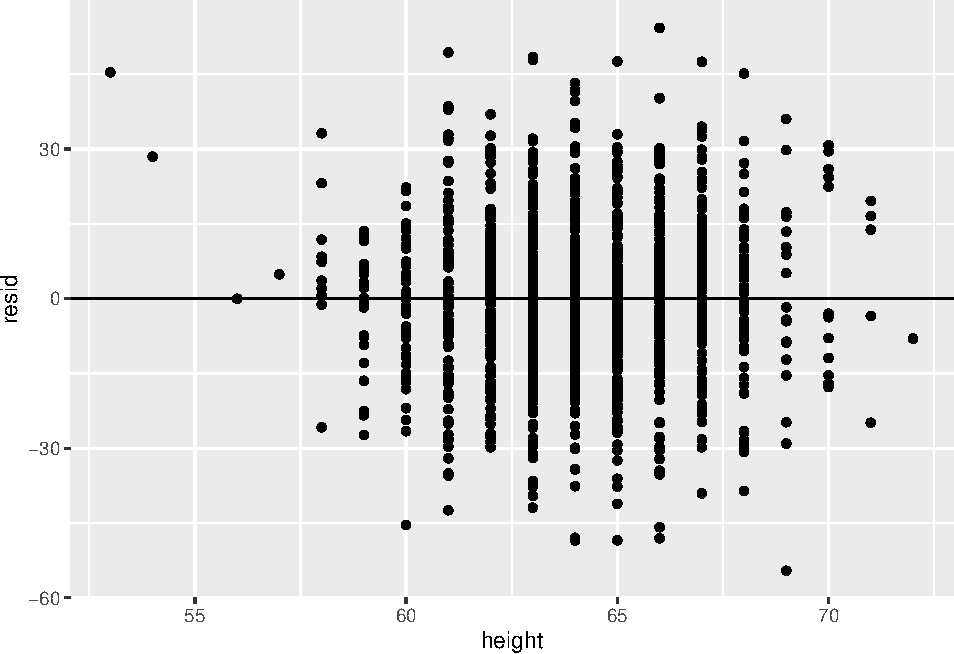
\includegraphics{lab-8-regression_files/figure-latex/unnamed-chunk-19-1.pdf}
Therefore, from the diagrams above, we can see that all the conditions
are met: from the qqplot we can see the residual nearly follows
normality and from residual plot we can see the variability is constant,
so we can use a linear regression.

\newpage

\begin{enumerate}
\def\labelenumi{\arabic{enumi}.}
\setcounter{enumi}{7}
\tightlist
\item
  Obtain a 95\% confidence interval for the coefficient on
  \texttt{gestation} and \texttt{age}. Interpret both confidence
  intervals.
\end{enumerate}

\begin{Shaded}
\begin{Highlighting}[]
\NormalTok{baby_model }\OperatorTok\StringTok{ }
\StringTok{  }\KeywordTok{summary}\NormalTok{()}
\end{Highlighting}
\end{Shaded}

\begin{verbatim}
## 
## Call:
## lm(formula = bwt ~ gestation + age + height + weight + parity, 
##     data = baby)
## 
## Residuals:
##     Min      1Q  Median      3Q     Max 
## -54.569 -10.506   0.453  10.063  54.285 
## 
## Coefficients:
##              Estimate Std. Error t value Pr(>|t|)    
## (Intercept) -86.59435   14.75733  -5.868 5.73e-09 ***
## gestation     0.46579    0.02992  15.568  < 2e-16 ***
## age           0.05233    0.08820   0.593   0.5531    
## height        1.04614    0.21064   4.967 7.82e-07 ***
## weight        0.06564    0.02584   2.540   0.0112 *  
## parity       -2.96394    1.16403  -2.546   0.0110 *  
## ---
## Signif. codes:  0 '***' 0.001 '**' 0.01 '*' 0.05 '.' 0.1 ' ' 1
## 
## Residual standard error: 16.35 on 1178 degrees of freedom
##   (52 observations deleted due to missingness)
## Multiple R-squared:  0.2106, Adjusted R-squared:  0.2072 
## F-statistic: 62.84 on 5 and 1178 DF,  p-value: < 2.2e-16
\end{verbatim}

\begin{Shaded}
\begin{Highlighting}[]
\NormalTok{z_cri <-}\StringTok{ }\KeywordTok{qnorm}\NormalTok{(}\FloatTok{0.025}\NormalTok{)}
\NormalTok{l1 <-}\StringTok{ }\FloatTok{0.46579} \OperatorTok{+}\StringTok{ }\NormalTok{z_cri}\OperatorTok{*}\FloatTok{0.02992}
\NormalTok{r1 <-}\StringTok{ }\FloatTok{0.46579} \OperatorTok{-}\StringTok{ }\NormalTok{z_cri}\OperatorTok{*}\FloatTok{0.02992}
\NormalTok{l1}
\end{Highlighting}
\end{Shaded}

\begin{verbatim}
## [1] 0.4071479
\end{verbatim}

\begin{Shaded}
\begin{Highlighting}[]
\NormalTok{r1}
\end{Highlighting}
\end{Shaded}

\begin{verbatim}
## [1] 0.5244321
\end{verbatim}

\begin{Shaded}
\begin{Highlighting}[]
\NormalTok{l2 <-}\StringTok{ }\FloatTok{0.05233} \OperatorTok{+}\StringTok{ }\NormalTok{z_cri}\OperatorTok{*}\FloatTok{0.08820}
\NormalTok{r2 <-}\StringTok{ }\FloatTok{0.05233} \OperatorTok{-}\StringTok{ }\NormalTok{z_cri}\OperatorTok{*}\FloatTok{0.08820}
\NormalTok{l2}
\end{Highlighting}
\end{Shaded}

\begin{verbatim}
## [1] -0.1205388
\end{verbatim}

\begin{Shaded}
\begin{Highlighting}[]
\NormalTok{r2}
\end{Highlighting}
\end{Shaded}

\begin{verbatim}
## [1] 0.2251988
\end{verbatim}

The 95\% confidence interval for coefficient on gestation is (0.4071479,
0.5244321), which means we are 95\% confident that the coefficient on
gestation is between 0.4071479 and 0.5244321.\\
The 95\% confidence interval for coefficient on age is (-0.1205388,
0.2251988), which means we are 95\% confident that the coefficient on
age is between -0.1205388 and 0.2251988.


\end{document}
